\documentclass{article}

\usepackage{graphicx}
\usepackage{amsmath}
\usepackage{courier}
\usepackage{float}
\usepackage{booktabs}

\begin{document}


\begin{titlepage}
\begin{center}


{\huge \textbf{COS 710: Assignment I}}

\vspace{1cm}

{\Large \textbf{Genetic Programming: Symbolic Regression}}

\vspace{1cm}

{\large u22498037 \\
University of Pretoria}

\vfill

\end{center}
\end{titlepage}

\tableofcontents

\section{Running Instructions}
To run the GP, a \texttt{makefile} is included as part of the submission. You can use the following commands in the directory to run the GP:

\begin{verbatim}
  make
  make run
\end{verbatim}

\section{Exploratory Data Analysis}
To better understand the data, analysis was done and a few graphs were plotted. By concatenating the dataset (figure \ref{fig:concat}), some initial intuition could assumed that the data is purely time-series (52 entries per year \(\implies\) 52 weeks), which is not unknown to regression problems.

\begin{figure}[H]
  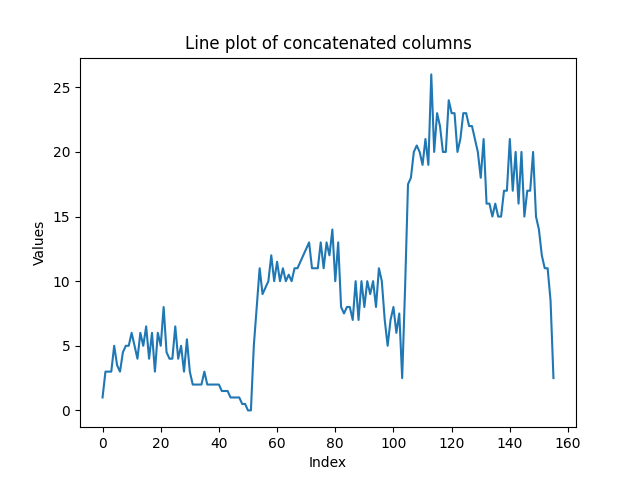
\includegraphics[width=\linewidth]{concatenated line plot.png}
  \caption{Concatenated line plot exploring if the dataset is possibly pure time-series.}
  \label{fig:concat}
\end{figure}

Alternatively, which turned out to be the right path, the variables contributed to the output with the question "given lugs from 1989 and lugs from 1990, what would the target, 1991, be?". As can be seen in Figure \ref{fig:independent}, each year were plotted separately against the target variable, which helped in understanding the dataset.

\begin{figure}[H]
  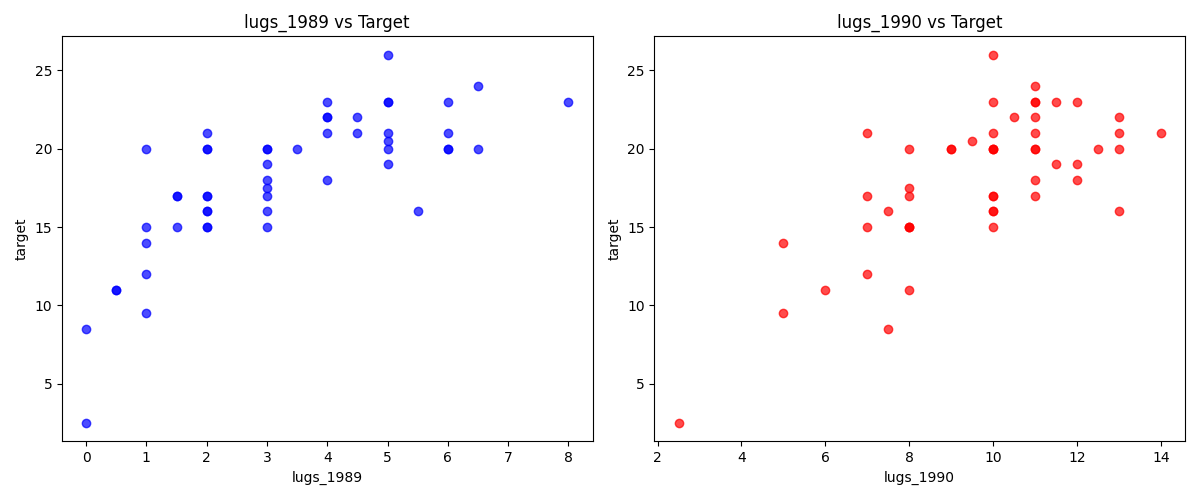
\includegraphics[width=\linewidth]{lugs vs target.png}
  \caption{Independent graphs explaining the relationship between lugs\_1989 vs target and lugs\_1990 vs target.}
  \label{fig:independent}
\end{figure}

\section{Pre-Processing}
For pre-processing, the data was normalised using min-max scaling \cite{patro_2015_normalization}:
\begin{equation}\label{norm}
  X' = \frac{X-min}{max-min}
\end{equation}
For this, the dataset was normalised column-wise to preserve features for each year. An extensive amount of experimentation was done with and without normalising to ensure that normalising was the better choice.
Experimentation was also done on normalising the entire dataset but since \texttt{lugs1989} and \texttt{lugs1990} approximately summed to the \texttt{target}, it meant that the \texttt{target}-variable determined the maximum value.

\section{GP Technical Specification}
\subsection{Structure}
\subsubsection{Function and Terminal Set}
\texttt{randomTerminal()} and \texttt{randomOperator()} functions determined which terminal or operator is chosen when generating a tree. For this reason, adding functions or operators heavily impacted the GP's performance since the selection of a function/terminal follows a uniform distribution.

Experiments included adding more \texttt{x1} and \texttt{x2} values to the terminal set increased the chance of an \texttt{x1} and \texttt{x2} being selected. This caused more valid trees but limited the diversity of floats included in the calculation (i.e. a float would only have 1/5th of a chance of being selected as a terminal).

Similarly, for the function set, more complex operators such as \(sin\), \(cos\), \(ln\),\(exp\),\(sqrt\),\(pow\) were experimented with but caused complex trees and couldn't converge sufficiently and performed badly. It must also be noted that no \(*\)-operator is included in the final function set because the GP experienced extremely large fitness values with complex trees.

This is the final set, given the reasoning and experimentation behind choosing the function and terminal set:
\begin{verbatim}
  F = {+, -, /, ln, sqrt}
  T = {double, x1, x2}
\end{verbatim}
where \texttt{double} is any float between -5.0 and 5.0.

\subsubsection{Train/test split}
An 80\%/20\% train split was used, but the training set consisted of the first 80\% of the data, and the testing set the last 20\% of the dataset.

\subsubsection{Initial Population}
The initial population was generated using grow method with \texttt{maxDepth} a generation-specific parameter. When a unary operator (e.g. \(ln\), \(exp\), \(sqrt\), \(pow\)) was randomly generated during the initial population, only a righthand subtree would be generated and the lefthand subtree would be nullified.

For each iteration, two booleans would independently determine if a left or right subtree would be further generated or not.

The following Pseudocode explains how the initial population is generated:

\begin{verbatim}
  generateIndividual(GPNode root, int maxDepth) {
    if (maxDepth is 0) {
      generateIndividual(root, 0)
      return
    }
    operator = randomOperator()
    root.isLeaf = false
    if (operator is not unary) {
      left = new GPNode
      right = new GPNode
      growLeft = probability of 0.5 or if maxDepth > 1
      growRight = probability of 0.5 or if maxDepth > 1
      if (growLeft is true) {
        generateIndividual(left, maxDepth-1)
      } else {
        generateIndividual(left, 0)
      }
      if (growRight is true) {
        generateIndividual(right, maxDepth-1)
      } else {
        generateIndividual(right, 0)
      }
    } else {
      left = nullptr
      right = new GPNode
      growRight = probability of 0.5 or if maxDepth > 1
      if (growRight is true) {
        generateIndividual(right, maxDepth-1)
      } else {
        generateIndividual(right, 0)
      }
    }
  }
  \end{verbatim}

\subsubsection{Tournament Selection}
For the selection method, a tried-and-trusted tournament selection has been used. This selection method selects \(n\) candidates to potentially apply genetic operators to. The candidate with the best fitness is selected as a parent.

\subsubsection{Mutation}
For the mutation genetic operator, a mix of approaches has been followed to ensure maximum diversity. A random point in the tree is chosen, and a random subtree (possibly just a leaf node) is generated and the subtree is replaced. This ensures that both grow and shrink mutation is possible with this approach. Root nodes can't be selected as well, and therefore 1 is added to the \texttt{mutationPoint} to prevent reproduction.

Throughout experimentation, not a lot of changes have been made to the mutation algorithm itself apart from setting the \texttt{mutationRate}.

\subsubsection{Crossover}
The crossover operator takes a standard approach by selecting random points in each parent, and then swops them around. The root nodes can't be swopped, which prevents unnecessary operations.

Throughout experimentation, not a lot of changes have been made to the crossover algorithm itself apart from setting the \texttt{crossoverRate}.

\subsubsection{Dropout}
This was an experimental feature, with inspiration from a neural network, but was short-lived due to its inefficiency in symbolic regression.

\subsubsection{Stopping Criteria}
For the stopping criterion, every GP run completed the full amount of generations (i.e. \texttt{maxGenerations}). No experimentation with early stopping or convergence testing has been done in this assignment.

\subsection{Parameter Fine-tuning}
At first, a lot (too much) of manual fine-tuning took place with a non-normalised dataset to get a feel for what is working and what is not. This was directed at maximising the Root Mean Squared Error (RMSE) which gives a true representation of how well the GP performed. After failure to accurately converge to a stable GP, parameter fine-tuning was used to identify a potential stable GP.

For parameter fine-tuning, an additional block of code has been run to test different combinations of parameters in order to get the lowest MSE. As a result, the best MSE was the combination of parameters with the lowest MSE.

To perform parameter fine-tuning, the algorithm iterated 100 times over randomly generated parameters. The parameters include:
\begin{itemize}
  \item Mutation Rate
  \item Crossover Rate
  \item Dropout Rate*
  \item Maximum Depth
  \item Population Size
  \item Maximum amount of Generations
  \item Tournament Size
\end{itemize}
\emph{*Not included in the final result, but briefly experimented with.}

\subsection{Fitness Function and Evaluation Methods}
\subsubsection{Fitness Function: MSE}
To evaluate the performance of the GP, Mean Squared Error (MSE) has been used as the \texttt{fitness()}-function. The reason behind this is that it can effectively capture good and bad trees and accurately represent trees' performance to improve the training process. The MSE function can be defined as follows:
\begin{equation}\label{mse}
  MSE(X) = \sum_{i=0}^{n} \frac{(f(x_i) - x_i)^2}{n}
\end{equation}

where \(X = \{x_0, x_1, ... , x_i\}\), \(n\) is the dataset size, \(f(x_i)\) is the fitness function, and \(x_i\) is the target value. In the training process, the attempt was to minimise \(MSE(X)\).
\subsubsection{Additional Evaluation Methods}
To ensure the GP converged sufficiently, additional measures helped to understand the GP performance better.

Before normalisation, the Root Mean Square Error (RMSE) helped to conceptualise the error by looking at the actual dataset. Intuitively, RMSE can be calculated by taking the square root of MSE: \(\sqrt{MSE(X)}\).

Additionally, R-Squared is a measure to express how good dependent variables is determined by the independent variables \cite{fernando_2024_rsquared}. This is done by calculating the variance of the dependent variables and the sum of squared errors from the independent variables. In this assignment, the following calculation was used:
\begin{equation}\label{norm}
  R^2(X) = 1 - \frac{\sum_{i=0}^{n} (x_i-f(x_i))^2}{\sum_{i=0}^{n} (x_i-\hat{x})^2}
\end{equation}
where \(\sum_{i=0}^{n} (x_i-f(x_i))^2\) is the sum of squared errors (SSE), and \(\sum_{i=0}^{n} (x_i-\hat{x})^2\) is the residual sum of squares (RSS). The R-squared measure helped to evaluate how well the GP performed across the testing dataset.

\section{Results and Interpretation}
After performing parameter fine-tuning, similar to Grid Search, a known technique in Machine Learning, these are the parameters for the best performing GP tree:
\begin{itemize}
  \item Population size: 54
  \item Number of generations: 98
  \item Crossover rate: 0.875687
  \item Mutation rate: 0.0703708
  \item Max Depth: 2
  \item Tournament Size: 7
\end{itemize}
which gave the following results (where run \(n\)'s seed \(i\) is \(i = n-1\)):
\begin{verbatim}
((x2 + x1) - (x1 * x2))
Testing Results
MSE: 0.014623
RMSE: 0.120927
R^2: 0.61293
\end{verbatim}

After training, the results were mostly consistent and acceptable with low MSE/RMSE. The \(R^2\) score, which explains the variance of a tree's performance, were negative in some of the runs, indicating that the tree performed worse than taking the mean alone. In general, over the 10 runs, the results were satisfactory (see appendix A for full report), showing good MSE/RMSE on the normalised dataset. Without normalising the dataset, however, it increased the difficulty to find a good GP solution to the dataset.

\begin{table}[H]
  \centering
  \resizebox{\textwidth}{!}{ 
  \begin{tabular}{lrrrrrrrr}
    \toprule
    & \multicolumn{4}{l}{\emph{Best Tree Statistics}} & \multicolumn{4}{l}{\emph{Population Statistics}} \\
    run & mean & min & max & std & mean & min & max & std \\
    \midrule
    0 & 0.059000 & 0.026948 & 0.105369 & 0.034107 & 10.428887 & 0.094734 & 130.345239 & 25.920744 \\
    1 & 0.102789 & 0.018198 & 0.135868 & 0.043319 & 2.352836 & 0.121347 & 8.455346 & 2.359953 \\
    2 & 0.032279 & 0.018806 & 0.046899 & 0.014107 & 1.262013 & 0.111640 & 6.872422 & 1.544866 \\
    3 & 0.014623 & 0.014623 & 0.014623 & 0.000000 & 1.173500 & 0.115792 & 7.822016 & 1.506081 \\
    4 & 0.014845 & 0.014623 & 0.018241 & 0.000872 & 1.730619 & 0.074554 & 34.575832 & 3.981563 \\
    5 & 0.033467 & 0.018198 & 0.135651 & 0.021558 & 1.105127 & 0.185363 & 5.333255 & 1.132751 \\
    6 & 0.062295 & 0.018590 & 0.101201 & 0.040841 & 1.057446 & 0.088766 & 6.952897 & 1.565298 \\
    7 & 0.023422 & 0.023422 & 0.023422 & 0.000000 & 7.323144 & 0.525170 & 61.094028 & 14.700151 \\
    8 & 0.019116 & 0.018198 & 0.029446 & 0.003096 & 4.536786 & 0.110300 & 91.681195 & 13.300235 \\
    9 & 0.130248 & 0.018481 & 0.135651 & 0.020009 & 0.727799 & 0.162884 & 2.784231 & 0.607410 \\
    \bottomrule
  \end{tabular}}
  \caption{Best Tree Fitness and Population Fitness statistics per GP run.}
  \label{resultsTable}
\end{table}

It is clear from Table \ref{resultsTable} that the GP performed well over multiple runs. In some cases (such as run 3 and run 7), it is observable that the best tree's standard deviation is 0.000, which simply means that the best tree was generated in the initial population and were preserved throughout all the generations.

Other observations also show that even though no elitism selection method was implemented, the best trees were preserved, even on bad occasions such as run 0's population fitness of 130.345239.

Overall, the results were consistent across multiple runs looking at the \emph{mean}-column from the \emph{Best Tree Statistics}.

\begin{figure}[H]
  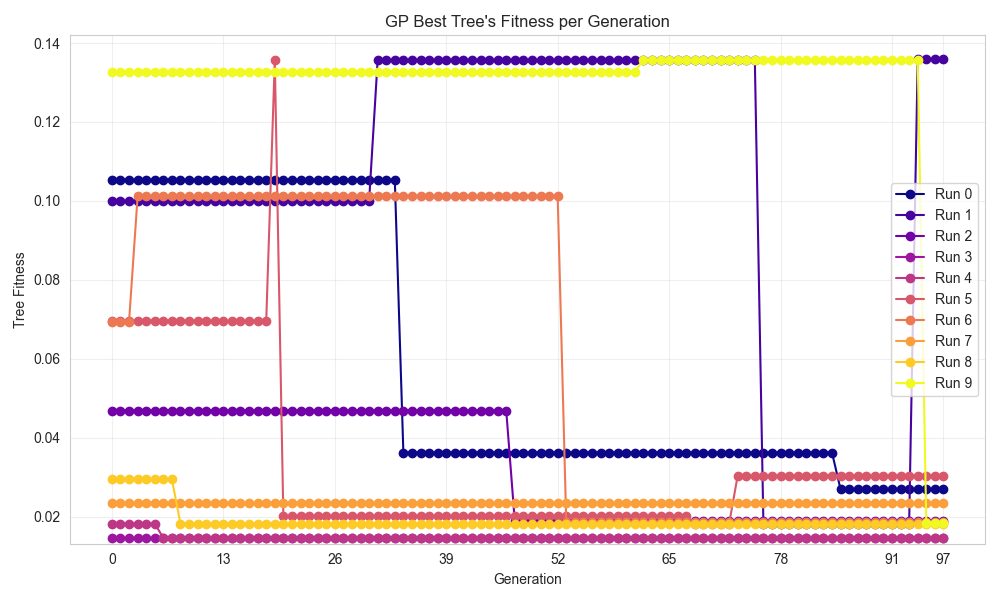
\includegraphics[width=\linewidth]{bestTree.png}
  \caption{GP Best Tree's Fitness per Generation over multiple runs explaining the convergence of the best tree.}
  \label{bestTree}
\end{figure}

Furthermore, it is observed in Figure \ref{bestTree} that the best tree is not entirely preserved but does get altered throughout the run. Although 0.14 is already satisfactory for the GP, the final states of each of the runs remained below 0.04 apart from Run 2.

\begin{figure}[H]
  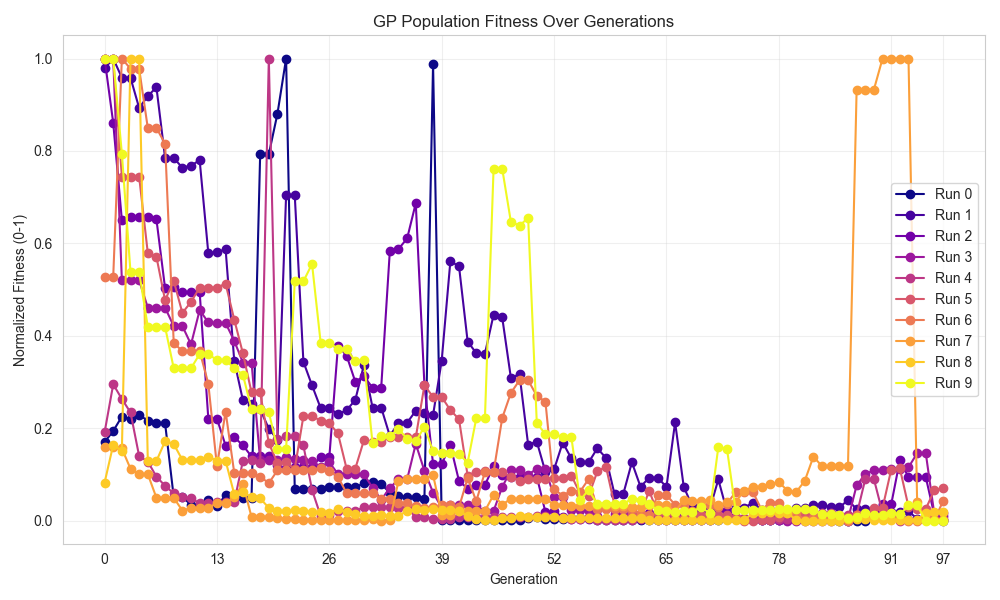
\includegraphics[width=\linewidth]{normalisedplot.png}
  \caption{GP's Normalised Population Fitness per Generation over multiple runs explaining convergence of the entire population.}
  \label{gppopFitness}
\end{figure}

Looking at the population fitness in Figure \ref{gppopFitness}, it is clear that there is some form of convergence. Up and to around generation 50, a lot of noise can be observed, followed by some stabilisation after generation 50. Run 7 experiences a sudden spike in population fitness close to the end, but fortunately manages to stabilise before the end of the run.

\section{Conclusion}
After taking some benchmarks from a normal Python regressor (using XGBoost), it was clear that this GP is far from perfect. The limited amount of data also possibly explained some difficulties experienced during the course of developing the symbolic regressor. A normal Python regressor is also more guaranteed for success since it fixes the input variables (in this case \texttt{lugs\_1989} and \texttt{lugs\_1990}) to weights and adds a singular bias in the form:
\[f(lugs\_1989, lugs\_1990) = a * lugs\_1989 + b * lugs\_1990 + c\]
where \(a\) and \(b\) are weights, and \(c\) the bias.
Trees in symbolic regression, are bad at keeping to a fixed function and simply try to stochastically find the best tree.

Other potential enhancements would include a more specific stopping criteria, as some populations experienced lower fitness before the stopping criteria and experienced worse fitness as a final result.

Nonetheless, the results were overall satisfactory and the GP converged well with a small amount of runs and performed well on both training and testing data, allowing it to generalise well and to not overfit.
\section{Appendix A: Raw Test Results}
\label{appendix:a}
\begin{verbatim}
  Best Tree Formula
  (((x2 + 0.760000) + ((x1 + x2) - x2)) - (x1 + x2))
  Testing Results
  MSE: 0.135868
  RMSE: 0.368603
  R^2: -2.596364
  ___________________
  Best Tree Formula
  ((x2 - x1) - (-0.930000 * x1))
  Testing Results
  MSE: 0.018806
  RMSE: 0.137134
  R^2: 0.502220
  ___________________
  Best Tree Formula
  ((x1 + x2) - (x1 * x2))
  Testing Results
  MSE: 0.014623
  RMSE: 0.120927
  R^2: 0.612930
  ___________________
  Best Tree Formula
  ((x2 + x1) - (x1 * x2))
  Testing Results
  MSE: 0.014623
  RMSE: 0.120927
  R^2: 0.612930
  ___________________
  Best Tree Formula
  (((x1 - (x2 + x1)) * x2) + (x2 + x1))
  Testing Results
  MSE: 0.030424
  RMSE: 0.174425
  R^2: 0.194689
  ___________________
  Best Tree Formula
  ((x2 * (x1 - x2)) + (0.140000 + x2))
  Testing Results
  MSE: 0.018590
  RMSE: 0.136344
  R^2: 0.507941
  ___________________
  Best Tree Formula
  ((0.090000 - x1) + (x2 + x1))
  Testing Results
  MSE: 0.023422
  RMSE: 0.153041
  R^2: 0.380043
  ___________________
  Best Tree Formula
  (x1 + (x2 - x1))
  Testing Results
  MSE: 0.018198
  RMSE: 0.134899
  R^2: 0.518317
  ___________________
  Best Tree Formula
  ((x2 + (((x2 * (x1 * x1)) - (x1 * x2)) * x2)) - (x1 - x1))
  Testing Results
  MSE: 0.018481
  RMSE: 0.135946
  R^2: 0.510807
  ___________________
\end{verbatim}

\bibliographystyle{IEEEtran}
\bibliography{COS710A1}

\end{document}
